% \section{Methodology}
% %\subsection{Motivation}
% % Previous works in Imprisonment Term Prediction (ITP) can be broadly classified into three categories (Section~\ref{rw} describe detailed related works). (1). {Language models}: These methods primarily capture textual information present in case descriptions to predict the sentencing term~\cite{devlin-etal-2019-bert,DBLP:conf/iclr/ClarkLLM20}. 
% % (2). {Models learning from previous cases}: Unlike the language model, this method aims to introduce historical sentencing data to infer the outcome of the current case~\cite{Rformer,DBLP:conf/cicai/ZhouLWKZW22}. 
% % (3). {Models equipped with legal knowledge}: Unlike the language model, this method introduces legal knowledge, such as law articles or explanations, to infer the outcome of the current case~\cite{neurjudge, ML-LJP}. 

% % Unfortunately, all these works towards the ITP problem have some drawbacks. Both \textit{language models} and \textit{models learning from previous cases} may suffer from imbalance and scarcity of training cases. The current \textit{models equipped with legal knowledge} makes it hard to do a deep understanding of the complex meanings of legal articles through plain text. Therefore, We need an effective method to extract and represent knowledge from legal statutes. 

% Prior studies~\cite{Greco2023BringingOI,wang-etal-2022-d2gclf} have validated the effectiveness of applying graphs to represent complicated semantic meanings and structures in text. Inspired by this, we propose a novel concept, namely \emph{law graph}, to effectively represent the structural information of law articles. Law graph is designed to include all essential components of a law article, including unlawful actions, severity classes, judicial outcomes, and their interconnections for judicial decision-making. Section~\ref{con} details the definition and construction of law graphs. 

% To leverage law graphs for ITP, we design a \underline{S}tatue \underline{K}nowledge \underline{E}ncoder (SKE) to convert the law graphs to machine-computable latent vector representations. 
% Section~\ref{lea} presents the detailed design of SKE. Furthermore, we elaborate on the ITP process by incorporating law graphs and SKE in Section~\ref{ee}.

% % to support the modeling of structural information of law articles and 
% % Given the ITP requirements, we propose a novel method, the law graph, to represent the statute structurally. Section~\ref{con} describes the construction process of the law graph. Then, in Section~\ref{lea}, we design a Statute Knowledge Encoder (SKE) to leverage the law graph representation for imprisonment term prediction. The end-to-end training process for ITP with law graph and SKE is discussed in Section~\ref{ee}.

% \KZ{According to ACL instructions,
% all captions must be placed below the table body.}
\begin{table}[t]
    \centering
    % \scriptsize
    \small
    \begin{tabular}{p{0.95\columnwidth}}
        \toprule
        {{\textit{Whoever commits any of the following acts to defraud a bank or any other financial institution of loans for the purpose of illegal possession shall}, {if the amount involved is substantial large}, \textbf{be sentenced to fixed-term imprisonment of not more than five years or criminal detention and shall also be fined not less than 20,000 yuan but not more than 200,000 yuan}; {if the amount involved is huge, or if there are other serious circumstances}, \textbf{shall be sentenced to fixed-term imprisonment of not less than five years but not more than 10 years and shall also be fined not less than 50,000 yuan but not more than 500,000 yuan}; {if the amount involved is extremely huge or there are other especially serious circumstances}, \textbf{shall be sentenced to fixed-term imprisonment of not less than 10 years or life imprisonment and shall also be fined not less than 50,000 yuan but not more than 500,000 yuan or be sentenced to confiscation of property}: \textit{(1) inventing false reasons for obtaining funds, projects, etc. from abroad; (2) using a false economic contract; (3) using a false supporting document; (4) using a false property right certificate as guaranty or repeatedly using the same mortgaged property as guaranty in excess of its value; or (5) defrauding loans by any other means.}}}\\
        \bottomrule
    \end{tabular}
    \caption{Example of legal norm theory in the Crime of Loan Fraud, Article 193 of the Criminal Law of China. \textbf{text}, \textit{text}, and {text}  refer to \textit{sanction}, \textit{hypothesis}, and \textit{disposition}, respectively.}
    % \KZ{Use colors sparingly. This pic looks a bit too colorful. Use colors in the same theme if possible.}}
    \label{tab:three}
    \vspace{-2em}
\end{table}

\section{\lawgraph{}} \label{con}
It is well-known that the legal rules are complicated to understand~\cite{zHodi2019limits}. The examples of legal terms presented in Section~\ref{int} illustrate that a single legal term may have distinct definitions in different legal rules, adding to the complexity. Additionally, Table~\ref{tab:three} highlights that statutory provisions are written with complex sentence structures, making legal texts arcane.

To capture the contextual meaning of statutory provision, the theory of legal norms~\cite{legalnorm,keuth1974some} suggests analyzing statutory provisions by breaking them down into three parts: the \textit{hypothesis} (which identifies illegal conduct), the \textit{disposition} (which categorizes the severity of the conduct), and the \textit{sanction} (which details the penalties). \tabref{tab:three} illustrates how these elements are represented within the statutory provision. 
%This approach aims to make legal rules easier to understand. 

However, even with this theory, legal rules remain hard to understand as each part is still a long and complex text. While complex, it is well-structured, as there are written rules for statutory provisions. For example, in China, there are Legislation Law and Legislative Technical Specifications~\footnote{\textit{Legislative Technical Specification (Trial) (I)}, which can be found at \url{http://zgfxqk.chinalaw.org.cn/portal/article/index/id/3045.html}.}. Drawing on previous research that shows the benefits of using graphs to explain complex ideas in text~\cite{Greco2023BringingOI,wang-etal-2022-d2gclf}, we propose a new method called \lawgraph{}. This approach is designed to leverage the clear and certain structure of laws by incorporating these three key components, making it easier to grasp the underlying principles of legal provisions.



\subsection{\lawgraph{} Definition} \label{dd}
We define a \lawgraph{} as $\mathcal{G}=\{\mathcal{V}, \mathcal{E}, \mathcal{T}_V, \mathcal{T}_E\}$, where $\mathcal{V}$ and $\mathcal{E}$ denote the set of nodes and edges, respectively. $\mathcal{T}_V$ and $\mathcal{T}_E$ denote node types and edge types, respectively. Each node $v\in \mathcal{V}$ is a pair node type and node value, i.e., $v=(v.value, v.type)$, where $v.type\in \mathcal{T}_V$. Each edge is a triplet $e=(v_i, v_j, e.type)\in \mathcal{E}$, where $e.type\in \mathcal{T}_E$. The node types and edge types are summarized in Table~\ref{tab:L_node_t} and \ref{tab:edge} and detailed in Appendix~\ref{app:e}. 
% Appendix~\ref{ne} shows the example nodes and edges. 
% \KZ{At this point give a snippet of a law graph, just a small fragment of it to illustrate of the diff types of nodes and edges you have talked about.}

% \paragraph{Vertex} We define four types of nodes representing different subjects and objects in the law article, demonstrated in Table \ref{tab:L_node_t}.

% \paragraph{Edge} Table \ref{tab:edge} shows the defined seven types of relations to connect the various nodes. 


\begin{table}
    \centering
    % \scriptsize
    \small
    \begin{tabular}{p{0.14\columnwidth}p{0.76\columnwidth}}
    \toprule
        Type & Definition\\
        \hline
        \textit{keyword} & A law keyword is the description selected from the statutory provisions.\\
        \hline
        \textit{punishment} & A law punishment represents sanction.\\
        \hline
        \textit{numerical} & An law numerical represents a limit on the amount of a description or punishment.\\
        \hline
        \multirow{2}{*}{\textit{Logic}} & \textit{And} denotes the conjunction of all child nodes.\\
        \cline{2-2}
        & \textit{Or} denotes the disjunction of the child nodes.\\
        \bottomrule
    \end{tabular}
    \caption{Node types in \lawgraph{}}
    \label{tab:L_node_t}
    \vspace{-1.5em}
\end{table}




\subsection{\lawgraph{} Construction}

We propose a rule-based method based on the written rules of statutory provisions to automatically construct the \lawgraph{} for each statutory provision. Following the legal norm theory, our method first splits each statutory provision into a \textit{hypothesis} component $H$ and pairs of \textit{disposition} $D$ and \textit{sanction} $S$ components, i.e., $\{(D_1, S_1), (D_2, S_2), ..., (D_n, S_n)\}$. For instance, we find the \textit{hypothesis} by rule-based searching for the keywords (``Whoever commits any of the following acts'', etc.) and punctuation, the \textit{disposition}-\textit{sanction} pairs by iteratively searching for the keywords (``if'', ``be sentenced to'', etc.).

Then, for each component, we design a parser to acquire the corresponding set of nodes and edges and construct a subgraph. After this, we connect all three subgraphs to construct the \lawgraph{}. As illustrated in Figure \ref{fig:law-graph-parser-structure} (a): First, we connect \textit{disposition} and \textit{hypothesis} by \textit{Constrain} relation; Then, we apply a logic node, either OR or AND, to connects nodes in the \textit{disposition} or \textit{hypothesis} subgraphs to the \textit{sanction} subgraph through the \textit{Satisfy} relation.
% \Kaiqi{Connect by what relation on which kinds of nodes?} 
A detailed example of converting the statutory provision in Table \ref{tab:three} from plain text into a \lawgraph{} is included in Appendix~\ref{sec:a}.
% \KZ{The descriptions of the three parsers and the pseudocode are too verbose! I don't think there's a lot of complexity technically in any of these parsers. Please use very concise words to describe these three parsers each in one paragraph (use examples if possible). No need the lengthy algorithms.}

\begin{table}
    \centering
    % \scriptsize
    \small
    \begin{tabular}{p{0.12\columnwidth} p{0.8\columnwidth}}
    \toprule
        Relation & Definition\\ 
        \hline
        \textit{Do} & The most general relation in the hypothesis part. It connects illegal conduct and the subject.\\
        \hline
        \textit{Default} & There is no meaning of the edge. It connects the component nodes of logical nodes.\\
        \hline
        \textit{Satisfy} & Connect the hypothesis and sanction part. It is only used when the law mentions it.\\
        \hline
        \textit{NextDo} &
        Connect two conducts, following the time order.\\
        \hline
        \textit{LeadTo} &
        Connect two causally related conducts.\\
        \hline
        \textit{Modify} &
        Connect the node with its modifier, which represents some attributes.\\
        \hline
        \textit{Constrain} &
        Connect the node and its constraining condition.\\
        \bottomrule
    \end{tabular}
    \caption{Edge types in \lawgraph{}.}
    \label{tab:edge}
    \vspace{-2em}
\end{table}

\begin{figure*}
    \centering    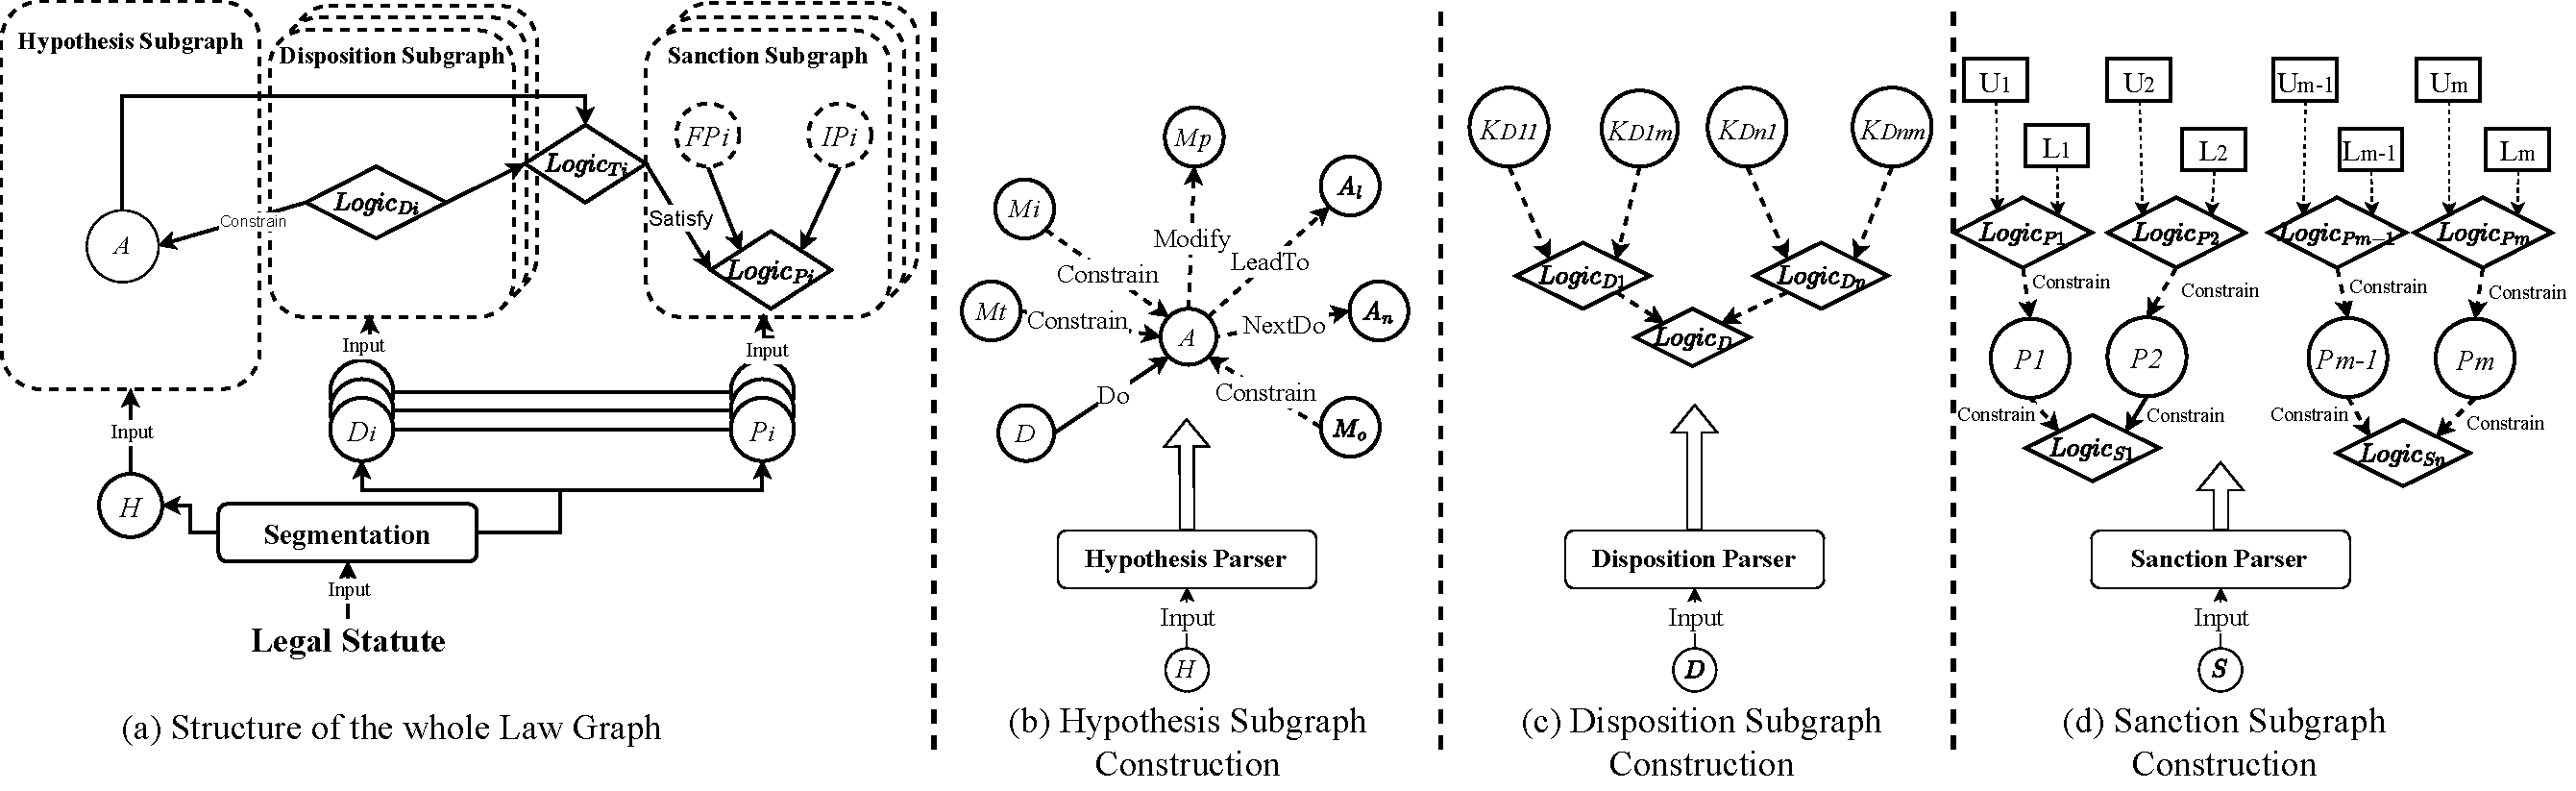
\includegraphics[width=\linewidth]{figs/Law Graph Structure.pdf}
    \caption{\lawgraph{} Parser Structure. The solid lines in the diagram represent edge that exist in all law graphs, while the dashed lines indicate edge that may not necessarily exist.
    % \KZ{This fig is not effective, very hard to understand, and takes up so much space. Need to revise or drop completely.}
    }
    \label{fig:law-graph-parser-structure}
    \vspace{-1.5em}
\end{figure*}

\textbf{Hypothesis Parser (HP).} The \textit{Hypothesis} parser finds the illegal conduct and related conditions outlined in a statutory provision. An illegal conduct contains the subject defendant $D$ and conduct $A$ while a condition includes the motivation $M_v$, the place $M_p$, the time $M_t$, the next conduct $A_n$, the lead conduct $A_l$, or other conditions $M_o$ of the provision. We obtain these elements from the given hypothesis text $H$ based on part-of-speech analysis~\cite{chiche2022part} and semantic parsing~\cite{lindemann-etal-2019-compositional} via Language Technology Platform (LTP) \cite{che-etal-2010-ltp}. 
For instance, in \tabref{tab:three}, $D$ is ``defendant'', $A$ is ``defraud a bank or any other financial institution of loans'', and $M_v$ is ``illegal possession''. 
After obtaining these elements, we create a graph node for each of them and connect all nodes according to \figref{fig:law-graph-parser-structure} (b). 
%belonging to conditions $O$ to the conduct $A$ by \textit{constrain} edge for $M_v, M_t, M_o$, i.e., $(M_o, A, Constrain)$; by \textit{modify} edge for $M_p$, $(M_p, A, Modify)$; by \textit{nextdo} edge for $A_n$, $(A_n, A, Nextdo)$; by \textit{leadto} edge for $A_l$, $(A_l, A, LeadTo)$. Besides, the subject defendant $D$ and conduct $A$ are connected by the \textit{do} edge, $(D, A, Do)$.


\textbf{Disposition Parser (DP).} 
% Given the disposition text $D$, we split it into several parts $\{D_1, D_2, \ldots, D_n \}$ by punctuation.
% Then, we input all disposition $\{D_1, D_2, \ldots, D_n \}$ to DP parser to obtain the nodes and edges.
% This rule-based parser target to extracts all dispositions $D = \{D_1, D_2, \ldots, D_n \}$ of input statutory provision.
A disposition often describes certain situations, such as ``the amount involved is substantially large'', ``the amount involved is huge, or if there are other serious circumstances'', etc., as illustrated in Table~\ref{tab:three}. We utilize prepositions ``or'' and ``and'' to further split each disposition $D_i$ into various situations $K_{Di} = \{K_{Di1}, \cdots, K_{Din} \}$. We create a node for each situation and a logic node for each preposition, then, connect them as illustrated in \figref{fig:law-graph-parser-structure} (c). For instance, in Table~\ref{tab:three}, $K_{D1} = $ \{``large amount''\}, and $K_{D2}$ has the edges (``large amount'', OR, \emph{Default}) and (``other serious circumstances'', OR, \emph{Default}). 
% \Kaiqi{What is the difference between D and K? Is K more concise? How do you make it more concise? by dropping some irrelevant words?}

% After obtaining these terms, we create a graph node for each of them and connect all nodes according to \figref{fig:law-graph-parser-structure} (c). 


\textbf{Sanction Parser (SP).} 
%Given the sanction text $S$, we split it into several sanctions $\{S_1, S_2, \ldots, S_n \}$ by punctuation. 
% parses all sanctions into $S = \{S_1, S_2, \ldots, S_n \}$. \Kaiqi{Should S be the input of this parser instead of output? SP parses all sanctions $S = \{S_1, S_2, \ldots, S_n \}$ to nodes and edges...}
%For instance, in Table~\ref{tab:three}, such as $S_2$ \textit{be sentenced to fixed-term imprisonment of not less than five years but not more than ten years and shall also be fined not less than 50,000 yuan but not more than 500,000 yuan}, etc. should be identified in this parser. 
Each sanction $S_i$ contains certain punishments $P = \{P_1, P_2, \ldots, P_m \}$, where each punishment $P_k$ has an upper bound $U_k$ and a lower bound $L_k$. SP parses these elements using keywords, such as ``fix-term imprisonment'', ``Fine'', and ``less than three years''. For instance, in Table~\ref{tab:three}, $P_1, P_4, P_7$ are ``fix-term imprisonment''; $P_3, P_5, P_8$ are ``fine''; and $P_2$, $P_7$ and $P_9$ are ``detention'', ``life imprisonment'' and ``confiscation of property'', respectively. Punishment $P_1$ has an upper bound ``less than five years'' and no lower bound. After obtaining these elements, we create a graph node for each of them and connect all nodes according to \figref{fig:law-graph-parser-structure}~(d). 

% The parser transforms the set of sanctions $S$ into a set of quadruplets (sanction, punishment, punishment upper bound, punishment lower bound) $\{(S_1, P_1, U_1, L_1), \ldots, (S_n, P_m, U_m, L_m) \}$. For instance, the parser transforms $S_2$, i.e., the second red text in \tabref{tab:three}, into two quadruplets ($S_2$, ``fixed-term imprisonment'', ``less than five years'', ``not more than ten years''), ($S_2$, ``Fine'', ``less than 50,000 yuan'', ``more than 500,000 yuan''), then generate nodes and relations according to sanctions' logic. \Kaiqi{So you generated one node for the whole quadruplet or one node for each element in the quadruplet? Also, we don't need to put $S_i$ in the quadruplet, only make it a triplet..}



\section{PTP with \lawgraph{s}}
The ``Satisfy'' relation in the proposed \lawgraph{s} plays a crucial role in connecting the hypothesis and disposition subgraphs to the corresponding sanction subgraph via a logic node $Logic_{Ti}$, as illustrated in Figure~\ref{fig:law-graph-parser-structure}. Since a legal rule often contains several disposition and sanction subgraphs, multiple $Logic_{Ti}$ nodes exist. If we aggregate information from all nodes regarding hypotheses and dispositions into $Logic_{Ti}$, the node will include all essential elements to make predictions. The possible predicted result resides in the sanction subgraph linked to the $Logic_{Ti}$ node. 
Inspired by this, we propose the Statute Knowledge Encoder (SKE). SKE applies a specialized message-passing mechanism to combine information from all nodes leading up to $Logic_{Ti}$, enhancing the ability of the model to learn the legal rules. For simplicity, we denote the set of  $Logic_{Ti}$ nodes as $\mathcal{V}_g\subset \mathcal{V}$.

\subsection{Statute Knowledge Encoder} \label{lea}

% In a \lawgraph{}, hypothesis, disposition and sanction are connected via the ``Satisfied'' edge. \Kaiqi{Since we are talking about law graph, why facts in the case matter?} The source node of the \textit{Satisfied} edge describes unlawful actions and their severity, and the target node is about the sanction outcome. For example, in Figure X\Kaiqi{add figure}, node number 14, labeled as ``OR'', is about a situation where someone tricks another party into getting something that is valued at a large amount. This node is linked to node number 4, which suggests that the tricking action could lead to a prison sentence of up to three years. When encoding the \lawgraph{}, we focus on the information in the nodes on the left side of the ``Satisfied'' edge. We denote these nodes as \textit{output nodes}, $n_o$. Then, $n_i$ denotes the \textit{source node} with outgoing edges alone. \Kaiqi{This is not clear. Make sure the notations are consistent.} In Figure X, node Z is the source node.  


% \KZ{This sentence repeats the preamble a little: We employ a message-passing mechanism that aggregates information from source nodes (i.e., nodes without incoming edges) to $\mathcal{V}_g$ in the \lawgraph{}.} 

The message-passing is start from source nodes, including $\{D, M_t, M_p, M_i, A_l, A_n, M_o, K_{Di}\}$, and end in $Logic_{Ti}$, in Figure~\ref{fig:law-graph-parser-structure}. %Appendix~\ref{sec:a} provides source nodes and output nodes example in the real \lawgraph{}.

\paragraph{Node Initialization} Except logic nodes, the value of a node $v\in \{v|v\in \mathcal{V} \land v.type\neq Logic\}$ can be represented by a set of words, i.e., $v.value=\{w_{v,1},\ldots,w_{v, N_{v}}\}$. We retrieve the word2vec~\cite{10.1145/3375395.3387641} embeddings of each word in the set and employ average pooling to obtain the initial node embeddings $h_{v}$: 
%have initial embeddings. \Kaiqi{Not clear what kind of initial embeddings.} One contains several words, $n_i=\{w_{n_i,1},\ldots,w_{n_i,|n_i|}\}$. Each word in the node has pre-trained word embedding. We apply Average Pooling, $Avg(\cdot)$, for all words embedding to obtain the node embedding (Equation~\ref{eq:node}), $h_{n_i} \in \mathbb{R}^{d}$. For all edges, we initialize them with random embedding, $h_{r} \in \mathbb{R}^{d}$.
\begin{equation}
    \mathbf{h}_{v} = \operatorname{Avg}(\{\mathbf{h}_{w_{v,1}},\ldots,\mathbf{h}_{w_{v,N_{v}}}\}),
    \label{eq:node}
\end{equation}
where $\mathbf{h}_{w_{v,j}} \in \mathbb{R}^{d}$ denotes the word embedding for the $j$-th word in node $v$.

\paragraph{Information Aggregation} Logic nodes behave differently in the message-passing process. The term "OR" signifies that only one of the requirements needs to be met, similar to a union, whereas "AND" indicates that all specified requirements must be satisfied, similar to an intersection. Consequently, following previous research~\cite{huang2022line}, we employ different aggregation operators for "OR" and "AND". Equations~\ref{eq:or} and \ref{eq:and} delineate the operations.
\begin{align}
\tilde{\mathbf{h}}_{v_j}^{(OR)} &= \max(\mathbf{m}_{1j},\ldots,\mathbf{m}_{|\mathcal{N}(v_j)|j}) \label{eq:or} \\
\tilde{\mathbf{h}}_{v_j}^{(AND)} &= \min(\mathbf{m}_{1j},\ldots,\mathbf{m}_{|\mathcal{N}(v_j)|j}) \label{eq:and} \\
\mathbf{m}_{ij} &= \mathbf{h}_{v_i} + \mathbf{h}_{e_{ij}}
\end{align}

% Each target vertex contains two parts of information: itself and its source vertices. 

\noindent where $\tilde{\mathbf{h}}_{v_j}^{(OR)}, \tilde{\mathbf{h}}_{v_j}^{(AND)} \in \mathbb{R}^{d}$ represent the embeddings of the logic nodes after aggregation, $\mathbf{m}_{ij}$ denotes the message obtained from the $i$-th incoming neighbor of node $v_j$, and $\mathbf{h}_{e_{ij}}$ denotes the embedding of the edge type linking $v_i$ and $v_j$. 
%The functions $\min(\cdot)$ and $\max(\cdot)$ represent the minimum and maximum pooling operations, respectively.

% \KZ{Be careful with the quotes: ` and ' or `` and ''.}
The aggregation for other nodes is akin to that of the ``OR'' node, as the node is not required to satisfy all incoming neighbors' conditions, for instance, conduct node $A$ in Figure~\ref{fig:law-graph-parser-structure}. The embeddings of non-logic nodes are obtained by:
\begin{equation}
\tilde{\mathbf{h}}_{v_j} = \max({\mathbf{h}_{v_j},\mathbf{m}_{1j},\ldots,\mathbf{m}_{|\mathcal{N}(v_j)|j}}).
\label{eq:nor}
\end{equation}

\begin{algorithm}[t]
\small
\caption{Statute Knowledge Encoder}
\label{alg:encoding}
\begin{algorithmic}[1]
\Require A \lawgraph{} $\mathcal{G}=(\mathcal{V}, \mathcal{E}, \mathcal{T}_V, \mathcal{T}_E)$. 
\Ensure Embedding of the $Logic_{Ti}$ nodes in $\mathcal{V}_g$. 
\State $\mathbf{h}_v \gets $ Equation \ref{eq:node} for all non-logic nodes $v$.
\State $\mathbf{h}_r \gets $ Initialize randomly for all edge types $r$.
\State $R \gets$ All edges in the hypothesis and disposition subgraphs in $\mathcal{G}$, sorted by in-degree. 
\While {$R$ is not empty}:
    \State Pop an edge \( e=(v_i, v_j, e.type) \) from \( R \)
    \State \( \mathbf{h}_{v_i} \gets \) Embedding(\( v_i \)) %\Comment{Get from $h_n$ if not processed}
    \State \( \mathbf{h}_{e_{ij}} \gets \) Embedding(\(e.type \)) %\Comment{Retrieve relation \( e_{ij} \)'s embedding}
    \State \( \mathbf{h}_{v_j} \gets \) Embedding(\( v_j \)) %\Comment{Get from $h_v$ if not processed}
    
    \State Update \( \mathbf{h}_{v_j} \) based on one of Equations~\ref{eq:or}, \ref{eq:and}, \ref{eq:nor} according to the type of $v_j$, i.e., $v_j.type$.
    %by \( (h_{v_i}, h_{e_{ij}}, h_{v_j}) \) 
    %\Comment{Update target node embedding}
    %\State Remove \( (v_i, e_{ij}, v_j) \) from \( R \)
\EndWhile
\State \textbf{Return} $\mathbf{h}_{v}$ for all $v\in \mathcal{V}_g$.
\end{algorithmic}
\end{algorithm}
% \vspace{-1.5em}


Algorithm~\ref{alg:encoding} outlines the process of encoding a Law Graph to obtain the embedding of nodes in $\mathcal{V}_g$. Since each node in $\mathcal{V}_g$ corresponds to one severity class, its embedding can then be utilized to match case facts, facilitating prison terms predictions.

\subsection{Prison Term Prediction} \label{ee}
It is widely recognized that illegal conducts of varying severity classes result in correspondingly different penalties. Therefore, we employ separate parameters for each severity class when matching with a case. Equation~\ref{eq:k} shows how to predict the prison term of a case based on one severity class:
\begin{align}
\hat{T}_{i,k} &= \textbf{W}^{k}_{t}\mathbf{h}_{i,k}, \label{eq:k} \\
\mathbf{h}_{i,k} &= \textbf{W}^{k}_{f}\left[\mathbf{h}_i; \mathbf{h}_{v,k}\right], \\
\mathbf{h}_i &= \text{Avg}({\mathbf{h}_{w_{i1}},\ldots,\mathbf{h}_{w_{i|F_i|}}}),
\end{align}
\noindent where $\textbf{W}^{k}_{t} \in \mathbb{R}^{1\times d}$ and $\textbf{W}^{k}_{f} \in \mathbb{R}^{d\times 2d}$ are two learnable weight matrices; $\mathbf{h}_{i,k} \in \mathbb{R}^{2d}$ denotes the combined representation of the $i$-th fact in the case and the $k$-th severity class; $\mathbf{h}_i \in \mathbb{R}^{d}$ is the representation of the $i$-th fact in the case; $\mathbf{h}_{v,k} \in \mathbb{R}^{d}$ is the embedding of the $k$-th nodes in $\mathcal{V}_g$ of \lawgraph{}; $\mathbf{h}_{w_{ij}} \in \mathbb{R}^{d}$ represents the embedding of the $j$-th word in the $i$-th fact. To be consistent, we utilize the same embedding methods as node initialization.

Then, we obtain the final prediction by summing up the prediction results for all severity classes,
\begin{equation}
\hat{T}_{i} = \sum_{k}\hat{T}_{i,k}.
\label{eq:f}
\end{equation}

% To ensure the predicted prison term closely aligns with the ground truth prison term ${T}_{i,k}$, 
We utilize the following loss function:
\begin{equation}
\mathcal{L} = \frac{1}{p}\sum_{i=1}^{p}(T_{i}-\hat{T}_{i})^2,
\label{eq:loss}
\end{equation}
\noindent where $p$ denotes the total number of training cases. 

